\documentclass{article}

\usepackage{mathtools}

\DeclarePairedDelimiter\abs{\lvert}{\rvert}%
\DeclarePairedDelimiter\norm{\lVert}{\rVert}%
\makeatletter
\let\oldabs\abs
\def\abs{\@ifstar{\oldabs}{\oldabs*}}

\usepackage[utf8]{inputenc}

\usepackage{tikz}
\usetikzlibrary{automata,arrows,positioning,calc}

\usepackage{subcaption}
\usepackage{gensymb}
\usepackage{amsmath,amsfonts,amssymb,amsthm,epsfig,epstopdf,titling,url,array}
\usepackage{enumerate}
\usepackage[a4paper, total={6in, 8in}]{geometry}

\usepackage{algorithm}
\usepackage[noend]{algpseudocode}

\makeatletter
\def\BState{\State\hskip-\ALG@thistlm}
\makeatother

\newcommand{\mathbbm}[1]{\text{\usefont{U}{bbm}{m}{n}#1}}
\newtheorem{thm}{Theorem}[section]
\newtheorem*{thmt*}{Theorem}
\newtheorem{lem}[thm]{Lemma}
\newtheorem{assumption}{Assumption}
\newtheorem{prop}[thm]{Proposition}


\newtheorem{defn}{Definition}[section]
\title{Homework 3 -- Xavier Gitiaux}
\author{}
\date{March 2019}

\begin{document}
\maketitle

\section{Exercise 1}

\subsection{Question a}
There are two hidden states $P$ and $A$:

\begin{center}
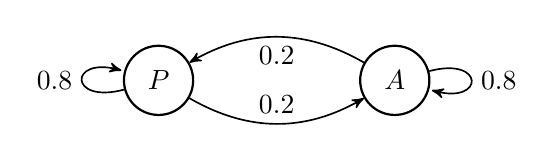
\begin{tikzpicture}[->, >=stealth', auto, semithick, node distance=3cm]
\tikzstyle{every state}=[fill=white,draw=black,thick,text=black,scale=1]
\node[state]    (ON)                     {$P$};
\node[state]    (OFF)[ right of=ON]   {$A$};
\path
 (ON) edge[loop left]   node{$0.8$}         (ON)
    edge[bend right] node{$0.2$}       (OFF)
    
 (OFF) edge[loop right]    node{$0.8$}                      (OFF)
	  edge[bend right]    node{$0.2$}    (ON);
\end{tikzpicture}
\end{center}

The prior distribution is $(0.5, 0.5)$. The transition matrix is
\begin{equation}
Q= \begin{pmatrix}
0.8 & 0.2 \\
0.2 & 0.8 \\
\end{pmatrix}
\end{equation}

\subsection{Question b}
There are four states: $P$, $A$, $C$ and $AC$. Since the lever are independent, the Markov structure is as follows:
$$P(A|A) = P[lever 1= ON|lever=1=ON]P[lever 2=OFF|lever2 = OFF]=0.56 = P[P|P]$$
$$P(A|P)= P[lever 1= ON|lever=1=OFF]P[lever 2=OFF|lever2 = OFF]=0.2 * 0.7 =  0.14= P[P|A]$$
$$P[C|C] = P[lever 1= OFF|lever=1=OFF]P[lever 2=ON|lever2 = ON] = 0.8 * 0.7 = 0.56 = P(AC|AC)$$
$$P(C|P) = P[lever 1= OFF|lever=1=OFF]P[lever 2=ON|lever2 = OFF] = 0.8 * 0.3 = 0.24 = P(P|C)$$ 
$$P(AC|A) = P[lever 1= ON|lever=1=ON]P[lever 2=OFF|lever2 = ON] = 0.8 * 0.3 = 0.24 = P(A|AC)$$ 
$$P(AC|P) = P[lever 1= ON|lever=1=OFF]P[lever 2=OFF|lever2 = ON] = 0.2 * 0.3 = 0.06 = P(P|AC)$$ 
$$P(C|AC) = P[lever 1= OFF|lever=1=ON]P[lever 2=ON|lever2 = ON] = 0.2 * 0.7 = 0.14 = P(AC|C)$$ 
$$P(C|A) = P[lever 1= OFF|lever=1=ON]P[lever 2=ON|lever2 = OFF] = 0.2 * 0.3 = 0.06 = P(A|C)$$ 


\begin{center}
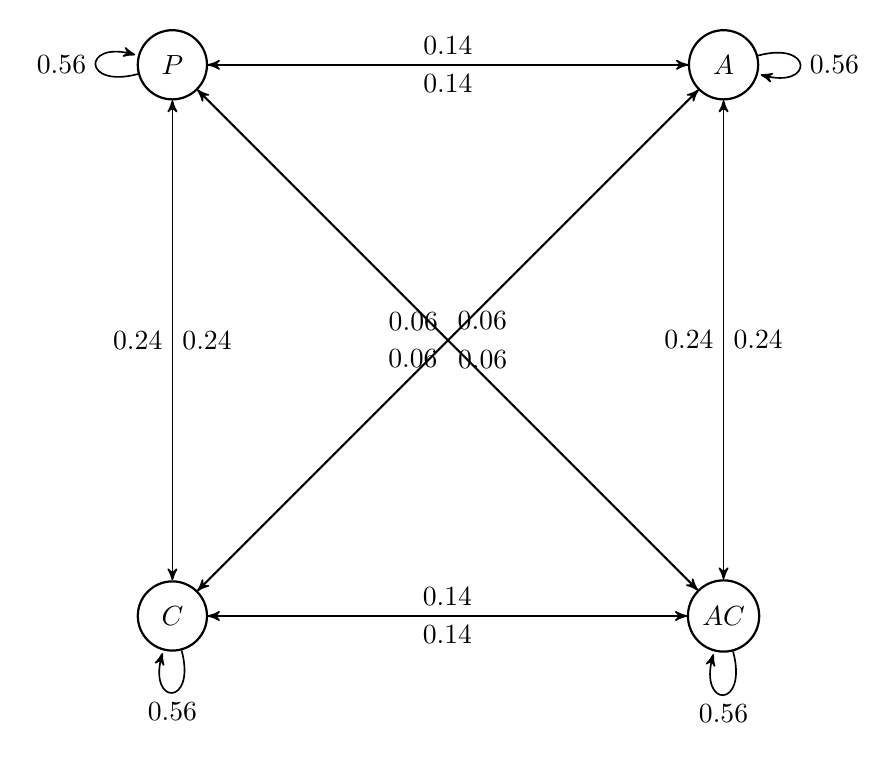
\begin{tikzpicture}[->, >=stealth', auto, semithick, node distance=7cm]
\tikzstyle{every state}=[fill=white,draw=black,thick,text=black,scale=1]
\node[state]    (P)                     {$P$};
\node[state]    (A)[right of=P]   {$A$};
\node[state]    (C) [below of=P]   {$C$};
\node[state]    (AC)[ right of=C]   {$AC$};
\path
 (P) edge[loop left]   node{$0.56$}         (P)
     edge node{$0.14$}       (A)
     edge   node{$0.24$}    (C)
     edge   node{$0.06$}    (AC)
 
 (AC) edge[loop below]   node{$0.56$}         (AC)
      edge   node{$0.24$}    (A)
      edge    node{$0.06$}    (P)
      edge    node{$0.14$}    (C)
 
 (C) edge[loop below]   node{$0.56$}         (C)
 	 edge  node{$0.24$}    (P)
 	 edge   node{$0.14$}    (AC)
 	 edge   node{$0.06$}    (A)
    
    
 (A) edge[loop right]    node{$0.56$}   (A)                   
     edge   node{$0.24$}    (AC)
     edge    node{$0.14$}    (P)
     edge    node{$0.06$}    (C);
\end{tikzpicture}
\end{center}

The prior distribution is $(0.25, 0.25, 0.25, 0.25)$. And the transition matrix is 

\begin{equation}
Q= \begin{pmatrix}
0.56 & 0.14 & 0.24 & 0.06 \\
0.14 & 0.56 &0.06 & 0.24 \\
0.24 & 0.06 & 0.56 & 0.14\\
0.06 & 0.24 & 0.14 & 0.56  \\
\end{pmatrix}
\end{equation}

\subsection{Question c}
\begin{equation}
P(P, A, AC, C) = P(P)P(A|P)P(AC|A)P(C|A)=(0.25)(0.14)(0.24)(0.06)=0.000504
\end{equation}

\subsection{d}
At time $1$:
\begin{equation}
\begin{split}
P(P|D, L) &\propto P(L|P)P(P|D) \\
& \propto P(P|D) \displaystyle\sum_{x_{2}}P(L|P, x_{2})P(x_{2}|P) \\
& \propto P(D|P)P(P) \displaystyle\sum_{x_{2}}P(L|x_{2})P(x_{2}|P) \\
& \propto (0. 8)(0.25) \left[(0.2)(0.56) + (0.4)(0.14) + (0.8)(0.24) + (0.9)(0.06)\right]\\
& \propto 0.207\end{split}
\end{equation}

\begin{equation}
\begin{split}
P(A|D, L) & \propto P(D|A)P(A) \displaystyle\sum_{x_{2}}P(L|x_{2})P(x_{2}|A) \\
& \propto (0. 6)(0.25) \left[(0.2)(0.14) + (0.4)(0.56) + (0.8)(0.06) + (0.9)(0.24)\right]\\
& \propto 0.258\end{split}
\end{equation}

\begin{equation}
\begin{split}
P(C|D, L) & \propto P(D|C)P(C) \displaystyle\sum_{x_{2}}P(L|x_{2})P(x_{2}|C) \\
& \propto (0. 2)(0.25) \left[(0.2)(0.24) + (0.4)(0.06) + (0.8)(0.56) + (0.9)(0.14)\right]\\
& \propto 0.0323\end{split}
\end{equation}

\begin{equation}
\begin{split}
P(AC|D, L) & \propto P(D|AC)P(AC) \displaystyle\sum_{x_{2}}P(L|x_{2})P(x_{2}|AC) \\
& \propto (0. 1)(0.25) \left[(0.2)(0.06) + (0.4)(0.24) + (0.8)(0.14) + (0.9)(0.56)\right]\\
& \propto 0.0181\end{split}
\end{equation}

After normalization $P(X_{1}|D, L)\approx (0.40, 0.50, 0.06, 0.04)$.

\bigskip
At time $t=2$, 
\begin{equation}
\begin{split}
P(X_{2}|D, L)& \propto P(L|X_{2}, D) P(X_{2}|D) \\
 & \propto P(L|P)\displaystyle\sum_{x_{1}}P(X_{2}|x_{1})P(D|x_{1})) \\ 
\end{split}
\end{equation}
Therefore 
$$P(X_{2}=P|D, L) = 0.2*\left[0.56*0.8 + 0.14*0.6+0.24*0.2 +0.06*0.1\right]=0.1172$$
$$P(X_{2}=A|D, L) = 0.4*\left[0.14*0.8 + 0.56*0.6+0.06*0.2 +0.24*0.1\right]=0.1936$$
$$P(X_{2}=C|D, L) = 0.8*\left[0.24*0.8 + 0.06*0.6+0.56*0.2 +0.14*0.1\right]=0.2832$$
$$P(X_{2}=AC|D, L) = 0.9*\left[0.06*0.8 + 0.24*0.6+0.14*0.2 +0.56*0.1\right]=0.2484$$
Therefore, after renormalization, $P(X_{2}|D, L)=(0.14, 0.23, 0.34, 0.29)$.


\end{document}